\subsection{SOC in cold atoms}
The methods of generating SOC in cold atoms are initially proposed in \cite{osterloh2005cold,ruseckas2005non}. It was first demonstrated in the observation of 1D SOC in a Bose-Einstein condensate \cite{lin2011spin}. Later, SOC was also realized in an atomic Fermi gas \cite{wang2012spin,cheuk2012spin}. Since then, a wide range of researches has been conducted or proposed in the field \cite{campbell2011realistic,wang2010spin,ho2011bose,cong2011unconventional,yu2011spin,bloch2012quantum,goldman2014light,jiang2011majorana,zhang2012collective,mancini2015observation,li2012quantum,anderson2012synthetic,beeler2013spin,stuhl2015visualizing,sugawa2018second,putra2020spatial}

In the first experimental realization of SOC in cold atoms \cite{lin2011spin}, the SOC Hamiltonian of neutral atoms  was engineered to be equivalent to an electronic system with equal contributions of the Rashba and the Dresselhaus couplings. 
\begin{equation}
    \hat{H}_{SOC} \propto k_x\sigma_y.
\end{equation}

In this neutral-atoms system, two internal hyperfine states $\ket{F,m_F}$ were selected to represent the pseudo-spin $\ket{\uparrow}$ and $\ket{\downarrow}$. And for a neutral atom, the internal electrons' spin is intrinsically coupled to the electrons' motion but the atomic spin is not coupled to the center-of-mass motion of the neutral atom. Here using lasers and magnetic fields, the researchers created coupling between the internal hyperfine states $\ket{\uparrow}$ and $\ket{\downarrow}$, and the momentum states of the neutral atoms.

% \begin{figure}[htbp]
%     \centering
%     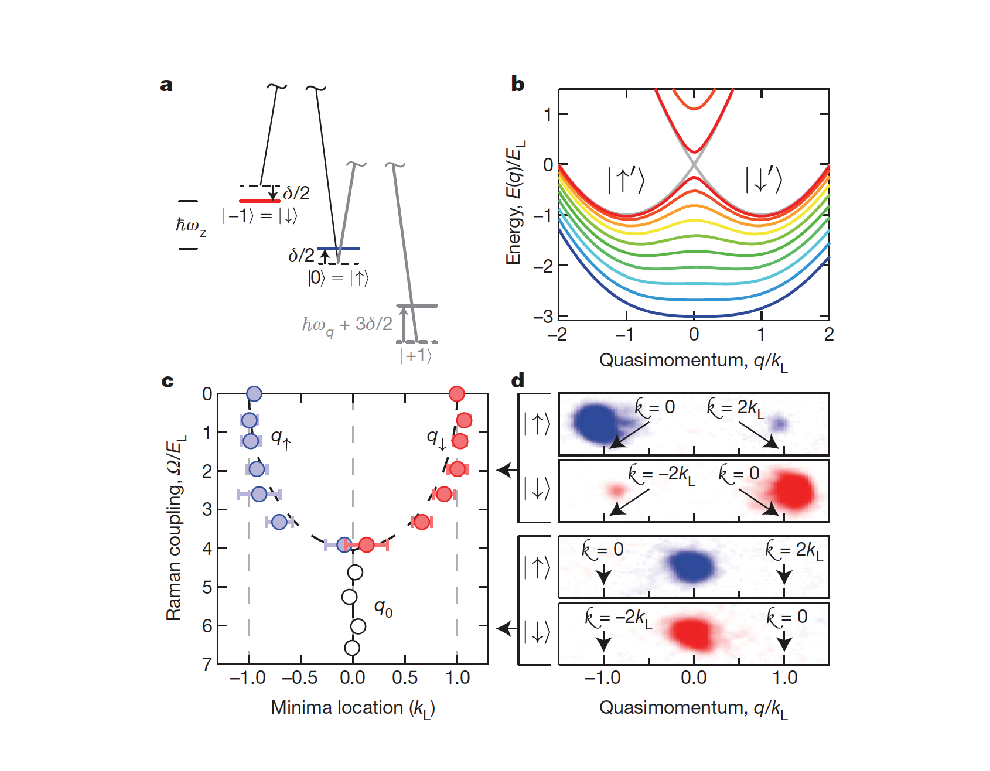
\includegraphics[width=\textwidth]{Chapter3_secs/SOCFIG1.pdf}
%     \caption{Fig.~1 in \cite{lin2011spin}, the scheme for creating SO coupling. }
%     \label{fig:SOC1}
% \end{figure}


Fig.~\ref{fig:Raman} and Fig.~\ref{fig:minima} show the scheme for creating SOC by using Raman coupling. In Fig.~\ref{fig:Raman}(b), the ${\rm ^{87}Rb}$ ground states $\ket{F=1,m_F=0,\pm 1}$ are coupled by a pair of Raman lasers with two-photon detuning $\delta$ relative to the Zeeman shift of states $\ket{F=1,m_F=0,\pm 1}$. Fig.~\ref{fig:minima}(a) is the dispersion relation of spin-orbit coupled atoms, energy vs quasi-momentum $q$ which is a good quantum number in the SOC system. Detailed discussions of the SOC Hamiltonian and quasi-momentum states are in Sec.~(\ref{Raman}). Also, SOC alters the mean-field interaction between quasi-momentum states in both energy bands, leading to two additional phases of a two-component BEC, the phase-mixed and the phase-separated. The phase transition was predicted and observed in \cite{lin2011spin, ji2014experimental}. Later the stripe phase was studied in more detail using the Bragg scattering signal \cite{putra2020spatial}. 